% !TEX program = pdflatex
\documentclass[11pt]{article}

% ---------- Page layout ----------
\usepackage[margin=1in]{geometry}

% ---------- Font and encoding ----------
\usepackage[T1]{fontenc}
\usepackage[utf8]{inputenc}
\usepackage{lmodern}
% ---------- Microtypography ----------
\usepackage{microtype}
\UseMicrotypeSet[protrusion]{basicmath} % fixes math symbol spacing


% ---------- Math packages ----------
\usepackage{amsmath, amssymb, mathtools}

% ---------- Lists and formatting ----------
\usepackage{enumitem}

% ---------- Figures and graphics ----------
\usepackage{graphicx}

% ---------- Hyperlinks ----------
\usepackage[hidelinks]{hyperref}

% ---------- Bibliography (biblatex) ----------
\usepackage[backend=biber,style=numeric,sorting=none,autocite=superscript]{biblatex}
\addbibresource{references.bib} % your .bib file
\AtEveryBibitem{\clearfield{doi}\clearfield{issn}\clearfield{isbn}}


% ---------- Line & paragraph spacing ----------
\usepackage{setspace}
\onehalfspacing
\setlength{\parskip}{0.75cm}

% ---------- Custom macros ----------
\newcommand{\E}[2]{E_{#1}^{#2}}   % energy: system, basis
\newcommand{\DE}{\Delta E}
\newcommand{\eps}{\varepsilon}

% Title info
\title{BSSE for Trimers: Expression, Term Analysis, and Study Plan}
\author{Prepared by Felix Rojas}
\date{\today}

% ---------- IncludeOnly ----------
% Compile *only* the first section:
\includeonly{
sections/01_trimer_bsse_expression,
sections/02_term_analysis,
sections/03_Computational_study_and_Number_of_total_computations,
sections/04_Project file layout_and_NWChem_job_plan
}
% You can add more, separated by commas:
% \includeonly{sections/01_trimer_bsse_expression,sections/02_term_analysis}

% ---------- Section number formatting ----------
\makeatletter
% Add dot after section numbers in headings
\renewcommand{\@seccntformat}[1]{\csname the#1\endcsname.\quad}
% Add dot after section numbers in TOC
\renewcommand{\numberline}[1]{#1.\hspace{0.5em}}
\makeatother

% =====================================================
\begin{document}
\maketitle

\begin{abstract}
A concise, modular document outlining the BSSE formulation for a trimer,
a short analysis of its terms, and the computational plan for our study.
\end{abstract}

\tableofcontents
\clearpage
% ---------- Modular sections ----------
\section{BSSE Expression for a Trimer}
\label{sec:expr}

Consider a molecular system composed of monomers \(A\), \(B\), and \(C\).
The total energy can be decomposed into one-, two-, and three-body contributions
following the many-body expansion formalism~\autocite{Valiron1997} :
\begin{align}
  \begin{split}
  E^{\mathrm{tot}}_{ABC} &=
  E_A + E_B + E_C 
  +   \varepsilon^{(2)}_{AB}
  +   \varepsilon^{(2)}_{AC}
  +   \varepsilon^{(2)}_{BC}
  +   \varepsilon^{(3)}_{ABC},\\[0.25cm]
  %--
  E^{\mathrm{tot}}_{ABC} &=
  \sum_{i}E_i + \sum_{i\neq j}\varepsilon_{ij}^{(2)} + \varepsilon^{(3)}_{ABC},
  \label{eq:manybody_trimer}
  \end{split}
\end{align}
where \(i,j\in\{A,B,C\}\) and the ordering \(ij\) is chosen so that \(i<j\)
to avoid double counting.
The two-body terms \(\varepsilon_{ij}^{(2)}\) refer to the interaction energy
between pairs of monomers, while the three-body term
\(\varepsilon_{ABC}^{(3)}\) represents the non-additive energy
that arises only when all three monomers are present simultaneously.
In other words, these terms correspond to the energy required to bring
two or three monomers together, respectively.

\noindent
The standard two-body interaction energy is defined as
\begin{align}
    \Delta E_{\mathrm{int}}^{\mathrm{st}}(ij)
    = \varepsilon_{ij}^{(2)}
    = E_{ij}^{\mathrm{tot}} - (E_i + E_j),
    \label{eq:equation_2}
\end{align}
and, analogously, the standard three-body interaction energy is
\begin{align}
    \Delta E_{\mathrm{int}}^{\mathrm{st}}(ijk)
    = \varepsilon_{ijk}^{(3)}
    = E_{ijk}^{\mathrm{tot}} - (E_i + E_j + E_k).
    \label{eq:st_three_body}
\end{align}

\noindent
By combining Eqs.~(\ref{eq:st_three_body}) and (\ref{eq:manybody_trimer}),
the total interaction energy of the system formed by monomers \(A\), \(B\), and \(C\)
can be expressed in two equivalent ways:
\begin{align}
      \Delta E_{\mathrm{int}}^{\mathrm{st}}
      &= E^{\mathrm{tot}}_{ABC} - \sum_{i}E_i,
      \label{eq:three_body_inter_1}\\[0.25cm]
      %--
      \Delta E_{\mathrm{int}}^{\mathrm{st}}
      &= 
          \varepsilon^{(2)}_{AB}
      +   \varepsilon^{(2)}_{AC}
      +   \varepsilon^{(2)}_{BC}
      +   \varepsilon^{(3)}_{ABC}.
      \label{eq:three_body_inte_2}
\end{align}

\noindent
Equation~(\ref{eq:three_body_inter_1}) is typically used when the total
cluster energy \(E^{\mathrm{tot}}_{ABC}\) and the monomer energies
\(E_A\), \(E_B\), and \(E_C\) are known from direct computation.
Equation~(\ref{eq:three_body_inte_2}), in contrast,
is more convenient when the two-body and three-body
interaction energies are determined separately, for example,
from potential energy surface calculations or incremental schemes.
%--
Thus, the interaction energy of the trimer system can be evaluated
either from the total energy of the cluster and its monomers,
or from the sum of the pairwise and three-body interaction contributions. In theory, if the ``exact'' energies of the monomers and the cluster were available, the interaction energy of a two-particle system could be determined exactly using Eq.~(\ref{eq:equation_2}).
In practice, however, this is not possible because all quantities are obtained through quantum-chemical approximations that depend on both the
\emph{level of theory}---such as Hartree--Fock (HF),
Møller--Plesset perturbation theory (MP2),
coupled-cluster theory with single, double, and perturbative triple excitations [CCSD(T)],
or density functional theory (DFT)---and the chosen \emph{basis set}
used to represent the molecular orbitals.


The fundamental problem that arises is one of \textbf{basis-set inconsistency}.
Within the framework of the variational principle and the
Roothaan--Hall approximation~\autocite{Mayer2003,Szabo2012}, molecular orbitals are expressed as
linear combinations of a finite set of \emph{basis functions}
(often referred to as atomic orbitals).
In this context, the total basis set of the supermolecule
is larger than that of the individual monomers:
the supermolecule basis consists of all basis functions
associated with every monomer in the system,
whereas each isolated monomer is described only by its own
subset of basis functions.
Consequently, the total energy of the cluster is evaluated in a
more complete variational space than that of the separated monomers.


If we compute the standard interaction energy of the \(AB\) cluster
under these conditions, we obtain
\begin{equation}
    \Delta E_{\mathrm{int}}^{\mathrm{st}}
      = E^{\mathrm{tot}}_{AB}(AB)
        - \big[E_{A}(A) + E_{B}(B)\big],
    \label{eq:st_basinconsistency}
\end{equation}
where the notation in parentheses explicitly denotes
the basis set employed for each subsystem.
Because the basis used for the cluster \((AB)\) is more extensive
than that used for the isolated monomers \((A)\) and \((B)\),
the total energy of the dimer is artificially stabilized.
As a result, the corresponding interaction energy
is spuriously lowered,
leading to what is known as the
\emph{basis set superposition error} (BSSE).

To correct for this basis-set inconsistency,
Boys and Bernardi~\cite{Boys1970} introduced the
\textit{counterpoise (CP) correction} procedure.
The method was originally formulated for a two-particle system (\(AB\)),
in which the total energy of the dimer \(AB\)
is evaluated in the full dimer basis \((AB)\),
and each monomer energy is recomputed in the same basis
while the partner monomer is replaced by \emph{ghost} orbitals
(i.e., basis functions without nuclei or electrons).
The counterpoise-corrected interaction energy is then defined as
\begin{equation}
    \Delta E_{\mathrm{int}}^{\mathrm{CP}}
      = E^{\mathrm{tot}}_{AB}(AB)
        - \big[E_{A}(AB) + E_{B}(AB)\big],
    \label{eq:CP_correction_two_body}
\end{equation}
%--
\noindent
where \(E_A(AB)\) and \(E_B(AB)\)
represent the monomer energies calculated in the presence of
the other monomer’s basis set.

%--
\clearpage
The BSSE quantifies how much the standard interaction energy is
\textit{contaminated} by basis-set inconsistencies.
A practical way to evaluate this contamination is to compute
the difference between the standard (uncorrected) interaction energy
and the counterpoise-corrected one\autocite{Duijneveldt1994} :
\begin{equation}
\label{eq:BSSE_definition_two_body}
\mathrm{BSSE}
= \Delta E_{\mathrm{int}}^{\mathrm{st}} - \Delta E_{\mathrm{int}}^{\mathrm{CP}}
= \big[E_{A}(AB)+E_{B}(AB)\big] - \big[E_{A}(A)+E_{B}(B)\big].
\end{equation}

\noindent
Since interaction energies for bound systems are typically negative (attractive), a \emph{negative} BSSE indicates that the uncorrected interaction energy, $\Delta E_{\mathrm{int}}^{\mathrm{st}}$, is \textit{too attractive}. After applying the counterpoise correction, the resulting interaction energy $\Delta E_{\mathrm{int}}^{\mathrm{CP}}$ is therefore \textbf{less negative}, and thus
\[
\mathrm{BSSE} < 0.
\]
This negative value represents the \textbf{fictitious stabilization}—the artificial energy lowering that arises purely from basis-set imbalance. Hence, the difference above quantifies how much of the apparent overbinding is due to BSSE.


One of the first extensions of the counterpoise (CP) correction to trimers was given by White and Davidson in their study of hydrogen-bonded ice\autocite{White1990}, and later generalized by Valiron and Mayer\autocite{Valiron1997}. In this framework, each two-body interaction energy $\varepsilon_{ij}^{(2)}$ ($i,j\in\{A,B,C\}$) is evaluated with CP as in Eq.~(\ref{eq:equation_2}) and assembled in Eq.~(\ref{eq:three_body_inte_2}). The remaining term,
$\varepsilon_{ijk}^{(3)}$, is the \emph{pure three-body} contribution. It is obtained from the many-body expansion for the trimer, Eq.~(\ref{eq:manybody_trimer}), with CP applied consistently to all monomer and dimer terms:
{\small
\begin{equation}
\label{eq:three_body_cp}
\begin{split}
\varepsilon_{ABC}^{(3)}(ABC)
= E^{\mathrm{tot}}_{ABC}(ABC)
- \Big[
  E_{A}(ABC) + E_{B}(ABC) + E_{C}(ABC)
  \\
  \qquad\qquad
  +\, \varepsilon_{AB}^{(2)}(ABC)
  +\, \varepsilon_{AC}^{(2)}(ABC)
  +\, \varepsilon_{BC}^{(2)}(ABC)
\Big].
\end{split}
\end{equation}
}
From here the (CP) interaction energy for the trimer can be written as
\begin{align}
    \begin{split}
        \Delta E_{\text{int}}^{\text{CP}} =
        \varepsilon_{AB}^{(2)}(AB) + \varepsilon_{AC}^{(2)}(AC) + \varepsilon_{BC}^{(2)}(BC) + \varepsilon_{ABC}^{(3)}(ABC)
    \end{split}
\end{align}
which can be arranged into the following 16-term expression by considering each contribution:
{\small
\begin{align}
    \begin{split}
        \Delta E_{\text{int}}^{\text{CP}} &=
        E_{AB}(AB) - \big[E_{A}(AB)+E_{B}(AB)\big] + E_{AC}(AC) -\big[E_{A}(AC)+E_{C}(AC)\big]\\
        &+  E_{BC}(BC)
        -\big[E_{B}(BC)+E_{C}(BC)\big]
        %--
        + \mathcal{E}_{ABC}
        \label{eq:equation-11}
    \end{split}
\end{align}
}
where 
\[
\mathcal{E}_{ABC} =  E_{ABC}(ABC) - \big[E_{AB}(ABC) + E_{AC}(ABC) + E_{BC}(ABC) - \big[E_{A}(ABC) + E_{B}(ABC)+E_{C}(ABC)\big]\big]
\]
%--
\clearpage
Now, the standard interaction energy  for the trimer is given by
\begin{equation}
    \Delta E_{\text{int}}^{\text{st}} = E_{ABC}(ABC) - \big[ 
    E_{A}(A) + E_{B}(B) + E_{C}(C)\big]
    \label{eq:equation-12}
\end{equation}
and from here the BSSE  is given by
\small{
\begin{align}
    \begin{split}
    \text{BSSE} &= \Delta E_{\mathrm{int}}^{\mathrm{st}} - \Delta E_{\mathrm{int}}^{\mathrm{CP}}\\[0.25cm]
    &=\Big[[E_{A}(AB) + E_{A}(AC)] -  [E_{A}(ABC) + E_{A}(A)]\Big]\\[0.25cm]
    %--
    &+\Big[[E_{B}(AB) + E_{B}(BC)] -  [E_{B}(ABC) + E_{B}(B)]\Big]\\[0.25cm]
    %--
    &+\Big[E_{C}(AC) + E_{C}(BC)] -  [E_{C}(ABC) + E_{C}(C)]\Big]\\[0.25cm]
    %--
    &+\Big[[E_{AB}(ABC) + E_{AC}(ABC)]-[E_{AB}(AB)+E_{AC}(AC)]\Big]
    %--
    + \Big[E_{BC}(ABC) - E_{BC}(BC)\Big]
    \end{split}
    \label{eq:equation-13}
\end{align}
}
\noindent





%\begin{align}
%    \begin{split}
%        \Delta E_{\mathrm{int}}^{\mathrm{CP}} =
        
%    \end{split}
%\end{align}







\section{BSSE for the Trimer System: Subset Representation}
\label{sec:bsse_trimer}

In the previous section we saw that the BSSE
[Eq.~(\ref{eq:equation-13})]
for a trimer depends on the monomer and dimer energies
evaluated in different basis sets.
If we define the set
\(\mathcal{B} = \{A,B,C\}\)
to represent the basis sets associated with each monomer,
we can describe the hierarchy of energy evaluations
in terms of the subsets of \(\mathcal{B}\).

\noindent
The \textbf{power set} of \(\mathcal{B}\),
denoted \(\mathcal{P}_{\mathcal{B}}\),
is the set of all possible subsets of \(\mathcal{B}\):
\[
\mathcal{P}_{\mathcal{B}}
   = \bigl\{
      \emptyset,
      \{A\},\{B\},\{C\},
      \{A,B\},\{A,C\},\{B,C\},
      \{A,B,C\}
     \bigr\}.
\]
The power set contains every possible combination of the basis sets,
including the empty set,
and its cardinality is given by
\[
|\mathcal{P}_{\mathcal{B}}| = 2^{|\mathcal{B}|} = 2^3 = 8.
\]

\noindent
We are interested in the subsets that contain a given element. So, for any element \(X \in \mathcal{B}\),
we can define the collection of all subsets that contain \(X\) as
\[
\mathcal{P}_{\mathcal{B}}(X)
   = \{\, S \subseteq \mathcal{B} \mid X \in S \,\}.
\]
For instance,
\[
\mathcal{P}_{\mathcal{B}}(A)
   = \{\{A\}, \{A,B\}, \{A,C\}, \{A,B,C\}\}.
\]
%--
\clearpage
This shows that each monomer (here \(A\)) appears in four different subsets of \(\mathcal{B}\). Then, every subset \(S\) of \(\mathcal{B}\) that contains \(A\) can be written uniquely as
\[
S = \{A\} \cup T,
\]
where \(T\) is any subset of \(\mathcal{B}\setminus\{A\}\).
Hence,
\[
\boxed{
\mathcal{P}_{\mathcal{B}}(A)
   = \bigl\{\, \{A\}\cup T \;\big|\;
     T\subseteq\mathcal{B}\setminus\{A\}\,\bigr\}.
}
\]
Now, we can see that there are \(2^{|\mathcal{B}|-1}\) possible subsets
\(T\subseteq\mathcal{B}\setminus\{A\}\),
it follows that
\[
|\mathcal{P}_{\mathcal{B}}(A)| = 2^{|\mathcal{B}|-1}.
\]
For a trimer (\(|\mathcal{B}|=3\)),
we have \( |\mathcal{P}_{\mathcal{B}}(A)| = 2^{2} = 4\),
corresponding exactly to the subsets
\(\{A\}\), \(\{A,B\}\), \(\{A,C\}\), and \(\{A,B,C\}\).

\noindent
In an analogous way, we can determine all subsets of
\(\mathcal{B}\) that contain a specific \emph{pair} of elements,
say \(A\) and \(B\).
These subsets correspond to all basis combinations
that simultaneously include both \(A\) and \(B\),
which are relevant for the evaluation of dimer energies.

\noindent
We define this collection as
\[
\mathcal{P}_{\mathcal{B}}(A,B)
   = \{\, S \subseteq \mathcal{B} \mid \{A,B\} \subseteq S \,\}.
\]
For our trimer example,
\[
\mathcal{P}_{\mathcal{B}}(A,B)
   = \{\{A,B\}, \{A,B,C\}\}.
\]
Each dimer therefore appears in exactly two subsets of \(\mathcal{B}\):
its own dimer basis and the full trimer basis. Following the same reasoning as before,
every subset \(S\) that contains both \(A\) and \(B\)
can be written uniquely as
\[
S = \{A,B\} \cup T,
\]
where \(T\) is any subset of the remaining elements,
\(\mathcal{B}\setminus\{A,B\}\).
Hence,
\[
\boxed{
\mathcal{P}_{\mathcal{B}}(A,B)
   = \bigl\{\, \{A,B\} \cup T
     \;\big|\;
     T\subseteq\mathcal{B}\setminus\{A,B\}\,\bigr\}.
}
\]
Because there are \(2^{|\mathcal{B}|-2}\) possible subsets
\(T\subseteq\mathcal{B}\setminus\{A,B\}\),
the number of subsets containing both \(A\) and \(B\) is
\[
|\mathcal{P}_{\mathcal{B}}(A,B)| = 2^{|\mathcal{B}|-2}.
\]
For the trimer (\(|\mathcal{B}|=3\)),
we obtain \( |\mathcal{P}_{\mathcal{B}}(A,B)| = 2^{1} = 2\),
corresponding to the subsets
\(\{A,B\}\) and \(\{A,B,C\}\),
as expected.

\noindent
More generally, for any \(k\)-tuple of elements
\(\{X_1, X_2, \ldots, X_k\}\subseteq\mathcal{B}\),
the collection of all subsets of \(\mathcal{B}\) containing these \(k\) elements
is given by
%--
\clearpage
\[
\boxed{
\mathcal{P}_{\mathcal{B}}(X_1,X_2,\ldots,X_k)
   = \bigl\{\, \{X_1,X_2,\ldots,X_k\} \cup T
     \;\big|\;
     T\subseteq\mathcal{B}\setminus\{X_1,X_2,\ldots,X_k\}\,\bigr\},
}
\]
with cardinality
\begin{equation}
|\mathcal{P}_{\mathcal{B}}(X_1,X_2,\ldots,X_k)|
   = 2^{|\mathcal{B}|-k}.
\label{eq:equation-14}
\end{equation}
This relation shows that:
\begin{itemize}[topsep=-0.25cm]
    \item each monomer (\(k=1\)) appears in \(2^{|\mathcal{B}|-1}\) subsets,
    \item each dimer (\(k=2\)) appears in \(2^{|\mathcal{B}|-2}\) subsets,
    \item each trimer (\(k=3\)) appears in \(2^{|\mathcal{B}|-3}\) subsets, and so on.
\end{itemize}
This hierarchical pattern is precisely what underlies
the structure of the BSSE corrections
in the Valiron--Mayer formulation of the many-body counterpoise method.



\noindent
This formalism provides a clear combinatorial interpretation
of the BSSE hierarchy:
each monomer must be evaluated in all subsets
that contain it,
while each dimer appears only in the subsets
that contain both of its monomers.
For the trimer case (\(N=3\)),
each monomer energy therefore involves
four basis sets
(its own, two dimer bases, and the trimer basis),
whereas each dimer energy appears in two
(its own and the trimer basis).
This subset structure offers a systematic and general framework
for expressing and counting the hierarchical counterpoise corrections
in any \(N\)-body cluster.


\section{Computational study and Number of total computations}
\label{sec:plan}

From the subset formalism in Sec.~\ref{sec:bsse_trimer}, the number of
primitive energy evaluations can be expressed compactly. Let $N$ be the
number of monomers. For each fragment size $k$ ($1\le k\le N$), there are
$\binom{N}{k}$ fragments, and each fragment must be evaluated in
$2^{N-k}$ supersets (all subsets that contain it). Thus,
\begin{equation}
N_{\mathrm{eval}}^{\mathrm{all\ terms}}(N)
= \sum_{k=1}^{N} \binom{N}{k}\,2^{\,N-k}.
\label{eq:Neval_all}
\end{equation}

However, when forming the \emph{BSSE} as the difference between the
counterpoise (CP) and standard interaction energies, the $N$-mer total
energy $E_{1\ldots N}(1\ldots N)$ cancels exactly. Therefore, the
$k=N$ term is not required:
\begin{align}
N_{\mathrm{eval}}^{\mathrm{BSSE}}(N)
&= \sum_{k=1}^{N-1} \binom{N}{k}\,2^{\,N-k}
\label{eq:equation-16}
\end{align}
%--
\clearpage
Recalling the binomial theorem\autocite{Beeler2015}, we have that
\[
(x+y)^{n}
  = \sum_{k=0}^{n} \binom{n}{k}\,x^{k}\,y^{\,n-k}.
\]
Thus,
\begin{equation*}
    3^{n}
    = (1+2)^{n}
    = \sum_{k=0}^{n} \binom{n}{k}\,1^{k}\,2^{\,n-k}
    = \sum_{k=0}^{n} \binom{n}{k}\,2^{\,n-k}.
\end{equation*}

\noindent
We can then re-write Eq.~(\ref{eq:equation-16}) by allowing the index
$k$ to range from $0$ to $N$. This defines a sum with $(N+1)$ terms,
that is, two more terms than the original.
These additional terms correspond to the first and last elements of
the full sum and must therefore be subtracted. Hence,
\begin{align*}
\sum_{k=1}^{N-1} \binom{N}{k}\,2^{\,N-k}
&=
\sum_{k=0}^{N} \binom{N}{k}\,2^{\,N-k}
 - \bigl(2^{N} + 1\bigr)
 = 3^{N} - \bigl(2^{N} + 1\bigr),
\end{align*}
where the term $2^{N}$ corresponds to the first term ($k=0$)
and the term $1$ corresponds to the last term ($k=N$).
In this way, we obtain
\begin{align}
N_{\mathrm{eval}}^{\mathrm{BSSE}}(N)
   = 3^{N} - \bigl(2^{N} + 1\bigr).
\label{eq:equation-18}
\end{align}

\noindent\textbf{For the trimer case ($N=3$)}, we have
\[
N_{\mathrm{eval}}^{\mathrm{BSSE}}(3)
= 3^{3} - 2^{3} - 1
= 27 - 8 - 1
= \boxed{18}.
\]
These 18 terms consist of:
\begin{itemize}[leftmargin=2em,topsep=-0.25cm]
  \item $12$ monomer-in-subset energies: each monomer appears in $2^{3-1}=4$ subsets,
        giving $3\times 4 = 12$;
  \item $6$ dimer-in-subset energies: each dimer appears in $2^{3-2}=2$ subsets,
        giving $3\times 2 = 6$.
\end{itemize}
If, in addition, one wishes to report the \emph{counterpoise (CP)},
the trimer total energy $E_{ABC}(ABC)$ must be included:
\[
N_{\mathrm{eval}}^{\mathrm{all\ terms}}(3)
= 18 + 1 = \boxed{19}.
\]

%--
\clearpage
%---
\subsection{Geometry sampling and scaling protocol}
\label{sec:families}

Each \emph{configuration} (geometry/scale) requires the counts above. 
Only the three isolated-monomer energies $E_A(A)$, $E_B(B)$, $E_C(C)$ 
are geometry independent and can be computed once per method/basis.

Hence, with $N_{\mathrm{geom}}$ geometries,
\[
\boxed{
\begin{aligned}
N_{\mathrm{runs}}^{\mathrm{BSSE}}(3)
  &= 3 \;+\; N_{\mathrm{geom}}\,[\,18-3\,]
   \;=\; 3 + 15\,N_{\mathrm{geom}},\\[4pt]
N_{\mathrm{runs}}^{\mathrm{all\ terms}}(3)
  &= 3 \;+\; N_{\mathrm{geom}}\,[\,19-3\,]
   \;=\; 3 + 16\,N_{\mathrm{geom}}.
\end{aligned}}
\]

In the trimer study we consider four shape families:
\emph{linear}, \emph{equilateral}, \emph{isosceles}, and \emph{scalene}
(Fig.~\ref{fig:figure-1}). 
For each family we sample $12$ similar (uniformly scaled) geometries, so
\[
N_{\mathrm{geom}} = 4 \times 12 = 48.
\]
Therefore,
\[
\boxed{
\begin{aligned}
N_{\mathrm{runs}}^{\mathrm{BSSE}}(3) 
  &= 3 + 15\times 48 \;=\; \mathbf{723},\\[2pt]
N_{\mathrm{runs}}^{\mathrm{all\ terms}}(3) 
  &= 3 + 16\times 48 \;=\; \mathbf{771}.
\end{aligned}}
\]

\begin{figure}[!ht]
  \centering
  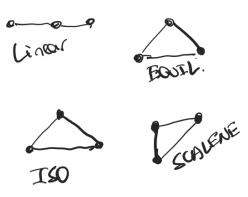
\includegraphics[width=0.28\linewidth]{images/trimers.png}
  \caption{Trimer shape families used for scaling: linear, equilateral, isosceles, and scalene.}
  \label{fig:figure-1}
\end{figure}

\subsection*{\centering Electronic-structure methods and basis sets}

All computations will be performed with three methods
(HF, MP2, CCSD(T)) and two basis sets
(aug-cc-pVDZ, aug-cc-pVTZ). If wall-time permits,
aug-cc-pVQZ will also be included. So, for $M=3$ (methods) and $B\in\{2,3\}$ (basis sets).
The total number of runs is
\[
\boxed{
\begin{aligned}
N_{\mathrm{runs}}^{\mathrm{BSSE}}(3; M,B)
  &= \bigl(3 + 15\,N_{\mathrm{geom}}\bigr)\; M B
   \;=\; \mathbf{723}\; M B,\\[4pt]
N_{\mathrm{runs}}^{\mathrm{all\ terms}}(3; M,B)
  &= \bigl(3 + 16\,N_{\mathrm{geom}}\bigr)\; M B
   \;=\; \mathbf{771}\; M B,
\end{aligned}}
\]
where $N_{\mathrm{geom}}=48$ for the four shape families
with 12 scale points each.

\noindent\textbf{With two basis sets ($B=2$):}
\[
\boxed{
\begin{aligned}
N_{\mathrm{runs}}^{\mathrm{BSSE}}(3)
  &= 723 \times 3 \times 2 = \mathbf{4338},\\[2pt]
N_{\mathrm{runs}}^{\mathrm{all\ terms}}(3)
  &= 771 \times 3 \times 2 = \mathbf{4626}.
\end{aligned}}
\]

\noindent\textbf{If aug-cc-pVQZ is added ($B=3$):}
\[
\boxed{
\begin{aligned}
N_{\mathrm{runs}}^{\mathrm{BSSE}}(3)
  &= 723 \times 3 \times 3 = \mathbf{6507},\\[2pt]
N_{\mathrm{runs}}^{\mathrm{all\ terms}}(3)
  &= 771 \times 3 \times 3 = \mathbf{6939}.
\end{aligned}}
\]




\section{Project file layout and NWChem job plan}
\label{sec:files}

\paragraph{Goals.}
(i) Minimize directory depth and enable a single parsing loop across outputs;
(ii) harvest \textbf{HF} and \textbf{MP2} energies from each \textbf{CCSD(T)} run to avoid redundant jobs;
(iii) keep runs fully reproducible and easy to re-generate.

\paragraph{Shallow, one-geometry-one-output (OGOO) layout.}
All geometry-specific work lives under
\texttt{\textless molecule\textgreater/\textless basis\textgreater/\textless shape\textgreater/s\textless 3-digit scale\textgreater/}:
\begin{verbatim}
<MOL>/<BASIS>/<SHAPE>/s001/
  run.nw     # all fragments + ghosts + all methods (SCF, MP2, CCSD(T))
  run.out    # single output to parse
  terms.csv  # aggregated row per geometry (energies + CP/BSSE)
\end{verbatim}
Here \texttt{<BASIS>} $\in$ \{\texttt{AVDZ}, \texttt{AVTZ}, \texttt{AVQZ}\}, and \texttt{<SHAPE>} encodes the trimer geometry family.
The directory name for the scale keeps your original convention \texttt{shape/s001}.

\paragraph{Monomer cache (geometry independent).}
Compute $E_A(A)$, $E_B(B)$, $E_C(C)$ once per basis and reuse:
\begin{verbatim}
<MOL>/cache/monomers/<BASIS>/
  monomers.nw   monomers.out   monomers.json
\end{verbatim}
This avoids repeating the same isolated-monomer optimizations for every geometry/scale.

\paragraph{Single-input strategy with method harvesting.}
For a given geometry, \texttt{run.nw} contains all fragment/basis-with-ghost tasks needed for CP on a trimer. Each task group is labeled with a unique \texttt{title} so parsers can grep reliably.
Each block runs, in order,
\begin{verbatim}
task scf
task mp2
task ccsd(t)
\end{verbatim}
so that \texttt{run.out} \emph{always} contains HF, MP2, and CCSD(T) energies for the same geometry and fragment/basis.
No per-method folders are needed; a single pass over \texttt{run.out} can collect all three methods.

\paragraph{Which energies are evaluated per geometry.}
If monomer self-energies are re-used from the cache, we evaluate $15$ geometry-specific terms per basis; if recomputed each time, there are $18$:
\begin{align*}
&\text{Monomers (cache or per-geometry): } E_A(A),\,E_B(B),\,E_C(C) \\
&\text{Monomers in ghosts: }
  E_A(AB),\,E_A(AC),\,E_A(ABC),\;
  E_B(AB),\,E_B(BC),\,E_B(ABC),\;
  E_C(AC),\,E_C(BC),\,E_C(ABC) \\
&\text{Dimers in their own basis: } E_{AB}(AB),\,E_{AC}(AC),\,E_{BC}(BC) \\
&\text{Dimers in trimer basis: } E_{AB}(ABC),\,E_{AC}(ABC),\,E_{BC}(ABC) \\
&\text{(Optional) Trimer: } E_{ABC}(ABC).
\end{align*}
Each quantity is captured for the three methods (SCF, MP2, CCSD(T)) from the \emph{same} output file.

\paragraph{Recommended file tags and parse keys.}
Prepend each block with a unique \texttt{title}, e.g.,
\texttt{title "E\_A(AB) : <MOL> <BASIS> <SHAPE> s001"},
so \texttt{terms.csv} can be populated by a single sweep over \texttt{run.out} using the tuple
\((\text{label}, \text{method})\) where \(\text{method} \in \{\text{SCF}, \text{MP2}, \text{CCSD(T)}\}\).
We standardize labels as strings like \texttt{E\_A(AB)}, \texttt{E\_AB(ABC)}, etc.

\paragraph{Minimal \texttt{run.nw} skeleton (per geometry).}
Below shows the pattern; repeat for each required fragment/basis-with-ghosts.
The \texttt{title} lines are the key to painless parsing.
\begin{verbatim}
start trimer_example
set print high
memory total 4000 mb

# --- Geometry with labeled fragments A, B, C ---
geometry units angstrom noautoz
  fragment A
    ...  # atoms of monomer A
  fragment B
    ...  # atoms of monomer B
  fragment C
    ...  # atoms of monomer C
end

# --- Basis blocks you'll switch between (AB, AC, BC, ABC) ---
basis "AB" spherical
  # define basis on A & B; use 'ghost' for centers not active
end

# ------------ E_A(AB): monomer A in AB basis (B as ghost) ------------
title "E_A(AB) : <MOL> <BASIS> <SHAPE> s001"
set geometry:fragment A
task scf
task mp2
task ccsd(t)

# ------------ E_AB(AB): dimer AB in AB basis ------------
title "E_AB(AB) : <MOL> <BASIS> <SHAPE> s001"
set geometry:fragment AB
task scf
task mp2
task ccsd(t)

# ------------ E_AB(ABC): dimer AB in ABC basis ------------
title "E_AB(ABC) : <MOL> <BASIS> <SHAPE> s001"
# define ABC basis (basis on all centers; ghost C for dimer AB if appropriate)
task scf
task mp2
task ccsd(t)

# ... repeat other required blocks ...
\end{verbatim}

\paragraph{Parser/CSV convention (single-loop friendly).}
\begin{itemize}[leftmargin=2em]
  \item \textbf{Key} each energy by \verb|(label, method)| where
        \verb|label \in {"E_A(AB)", "E_AB(ABC)", ...}| and
        \verb|method \in {"SCF","MP2","CCSD(T)"}|.
  \item \textbf{Row schema} for \texttt{terms.csv} (per geometry):\\
  \texttt{mol,basis,shape,scale, E\_A(A)\_SCF, E\_A(A)\_MP2, E\_A(A)\_CCSDT, ..., E\_AB(ABC)\_CCSDT, E\_ABC(ABC)\_CCSDT, CP\_interaction(method), BSSE(method)}
  \item \textbf{Reuse} the cached $E_A(A)$, $E_B(B)$, $E_C(C)$ columns by basis from\\
        \texttt{<molecule>/cache/monomers/<basis>/monomers.json}.
\end{itemize}

\paragraph{Automation hook.}
Alongside \texttt{run.nw}, store \texttt{geom.json} with Cartesian coordinates and the scale tag (e.g., \texttt{s001}).
A Python driver:
(i) builds \texttt{run.nw} from \texttt{geom.json} and a template,
(ii) executes NWChem,
(iii) parses HF/MP2/CCSD(T) energies keyed by \texttt{title} lines,
(iv) computes CP-corrected interaction energies and BSSE per method, and
(v) appends a row to \texttt{terms.csv}.
This preserves your original workflow while enabling a single over-the-tree parsing loop.


% ---------- Appendices ----------
\clearpage
\appendix
\numberwithin{equation}{section} % Eq. numbering A.1, A.2, ...

% appendices/A1_trimer_cp_derivation.tex

\section{Trimer CP-Corrected Interaction Energy: Algebraic Derivation}
\label{app:trimer-cp-derivation}

\subsection*{Definitions}
CP two-body (evaluated in each dimer basis with ghost functions):
\begin{align}
\varepsilon_{ij}^{(2)}(ij)
&= E_{ij}(ij) - \big[E_i(ij)+E_j(ij)\big],
\qquad i,j \in \{A,B,C\}.
\label{app:eq:cp-dimer}
\end{align}
CP three-body (pure term in the trimer basis):
\begin{align}
\varepsilon_{ABC}^{(3)}(ABC)
&= E_{ABC}(ABC)
 - \Big( E_{AB}(ABC)+E_{AC}(ABC)+E_{BC}(ABC)
 - [E_A(ABC)+E_B(ABC)+E_C(ABC)] \Big).
\label{app:eq:cp-three}
\end{align}

\subsection*{CP interaction energy for the trimer}
\begin{align}
\Delta E_{\mathrm{int}}^{\mathrm{CP}}
&= \varepsilon_{AB}^{(2)}(AB) + \varepsilon_{AC}^{(2)}(AC) + \varepsilon_{BC}^{(2)}(BC)
   + \varepsilon_{ABC}^{(3)}(ABC) \notag\\
&= \big[ E_{AB}(AB) - E_A(AB) - E_B(AB) \big]
 + \big[ E_{AC}(AC) - E_A(AC) - E_C(AC) \big] \notag\\
&\quad + \big[ E_{BC}(BC) - E_B(BC) - E_C(BC) \big]
 + \varepsilon_{ABC}^{(3)}(ABC).
\label{app:eq:cp-trimer}
\end{align}

\subsection*{Standard interaction energy}
\begin{align}
\Delta E_{\mathrm{int}}^{\mathrm{st}}
= E_{ABC}(ABC) - \big[ E_A(A)+E_B(B)+E_C(C) \big].
\label{app:eq:std-trimer}
\end{align}

\subsection*{BSSE (convention)}
We define
\[
\mathrm{BSSE} = \Delta E_{\mathrm{int}}^{\mathrm{st}} - \Delta E_{\mathrm{int}}^{\mathrm{CP}}.
\]
Algebraic grouping yields
\begin{align}
\label{app:eq:bsse-trimer-grouped}
\mathrm{BSSE}
&=\Bigl( E_{A}(AB)+E_{A}(AC) - E_{A}(ABC) - E_{A}(A) \Bigr) \notag\\
&\quad+ \Bigl( E_{B}(AB)+E_{B}(BC) - E_{B}(ABC) - E_{B}(B) \Bigr) \notag\\
&\quad+ \Bigl( E_{C}(AC)+E_{C}(BC) - E_{C}(ABC) - E_{C}(C) \Bigr) \notag\\
&\quad+ \Bigl( E_{AB}(ABC) - E_{AB}(AB) \Bigr)
      + \Bigl( E_{AC}(ABC) - E_{AC}(AC) \Bigr)
      + \Bigl( E_{BC}(ABC) - E_{BC}(BC) \Bigr).
\end{align}

\noindent
Equivalently, the fully expanded form (18 terms) is obtained by distributing the
grouped differences in Eq.~\eqref{app:eq:bsse-trimer-grouped}.
   

% ---------- Bibliography (optional for now) ----------
\printbibliography

\end{document}
